\chapter{Research Methods}
The methods (data collection and analysis techniques) you used to solve your research question are described in this chapter. You will usually need to refer back to texts in your literature survey to justify the techniques that you have chosen to solve your particular research problem. 

\section{Research Techniques}
In a survey or case study project, these might include, for example, the questionnaires and/or interview scripts. In a project which requires development or experimentation, the development of the code or mock-ups is discussed.

\subsection{Presenting Figures}
Note that every Figure and table should be referred to in the text. Here I am referring to Figure 3.1 in Microsoft Word by choosing Insert -> Reference -> Cross-Reference ->Figure and insert reference to only number and label. Because I used the Word Insert Caption feature, it means I can insert cross references in the text that are updated automatically and the table of figures can be updated automatically.

\begin{figure}[h]
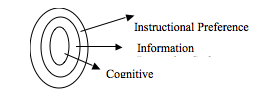
\includegraphics	{diagram1.png}
\caption{Curry's Onion Model}
\end{figure}

\subsection{Presenting Tables}
Tables and references to tables are done in the same way (see Table 3.1).  
\begin{table}[h]
	\begin{tabular}{| p{3.6cm} | p{3.6cm} | p{3.6cm} | p{3.6cm} |}
	\hline
	& Cognitive Personality Style  (CPS) & Information Processing Style  (IPS) & Instructional Preference  (IP) \\ \hline
	Cognition-centred Approach & Examines underlying cognitive traits\index{cognitive traits} in internal cognitive activities & Examines underlying cognitive traits in information processing of external stimuli & Extrapolates from CPS and IPS adopting a cognition perspective to predict preference in instruction \\ \hline
	\end{tabular}
\caption{Mapping between different approaches and their goals}
\end{table}

Table 3.1 illustrates how tables should be presented in your dissertation. 

\subsection{Presenting Bulleted Lists}
You may wish to use bullet points for a list, if the items in the list are:

\begin{itemize}
	\item short.
	\item closely related to each other.
\end{itemize}

However, you should not use bullet points as an alternative to correctly written English. 
